\section{Parametrized Neural Network}
\subsection{Discriminating Masses}
In figure \ref{fig:PNNDist} I have drawn the distribution of the output from the trained \ac{PNN} architecture 
(see section \ref{subsec:PNNArch}). The model was trained using the FS-MLM data set. In figure \ref{fig:PNNDist},
4 signals have been included; ($\tilde{\chi}_1=50$, $\tilde{\chi}_2=250$GeV), ($\tilde{\chi}_1=100$, $\tilde{\chi}_2=200$GeV), 
($\tilde{\chi}_1=200$, $\tilde{\chi}_2=300$GeV) and ($\tilde{\chi}_1=150$, $\tilde{\chi}_2=250$GeV). All data, including 
both signal and background were given the values of $50$ and $250$. As was the hope, the \ac{PNN} performs better on 
the signal for which the parameter choice was correct ($50-250$) and worse on the rest. This means
that the \ac{PNN} model is tuned to each signal combination.
\begin{figure}
    \makebox[0.95\linewidth][c]{%
    \centering
    \begin{subfigure}{.45\textwidth}
        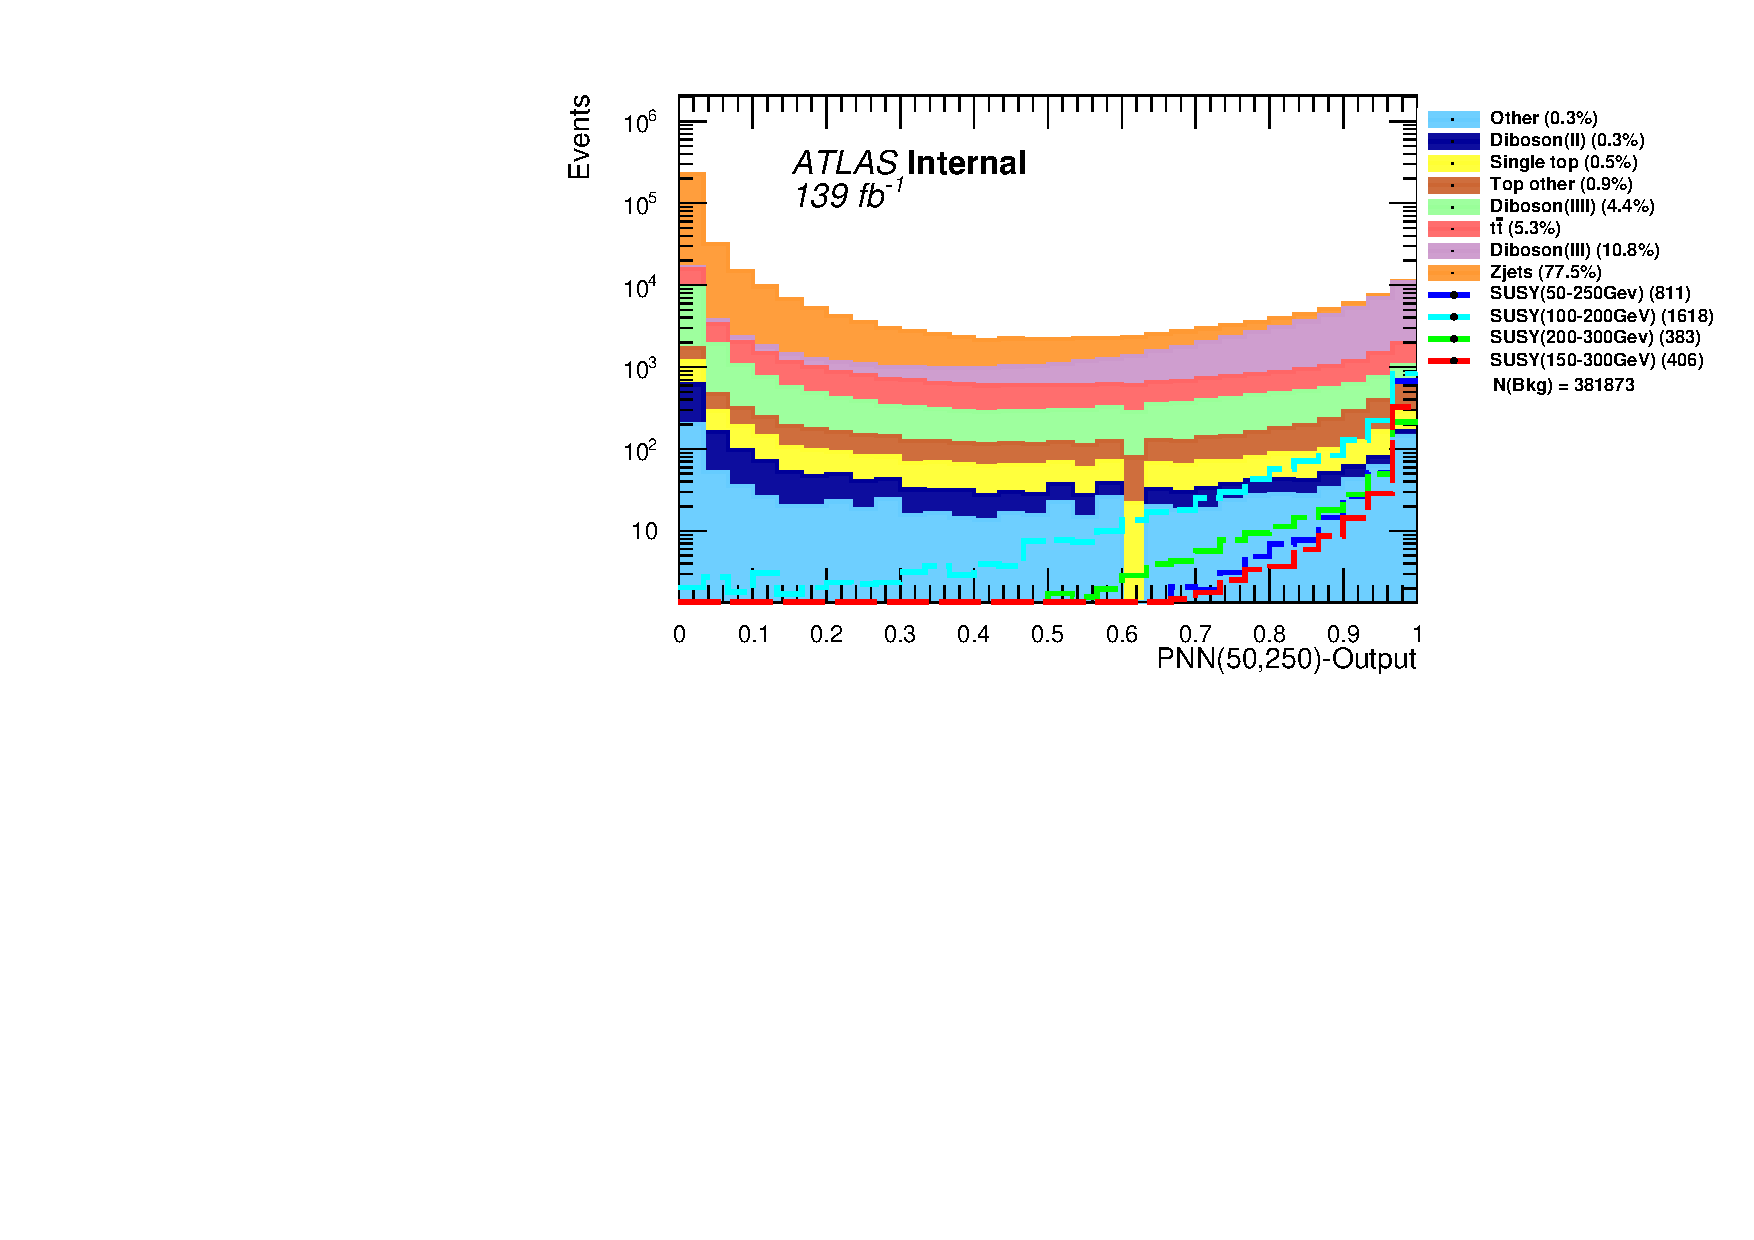
\includegraphics[width=\textwidth]{Figures/MLResults/NN/SUSY/MLDist/PNNDistTest/PNN50250Dist.pdf}
        \caption{}
        \label{fig:PNN50250Dist}
    \end{subfigure}
    \hfill
    \begin{subfigure}{.45\textwidth}
        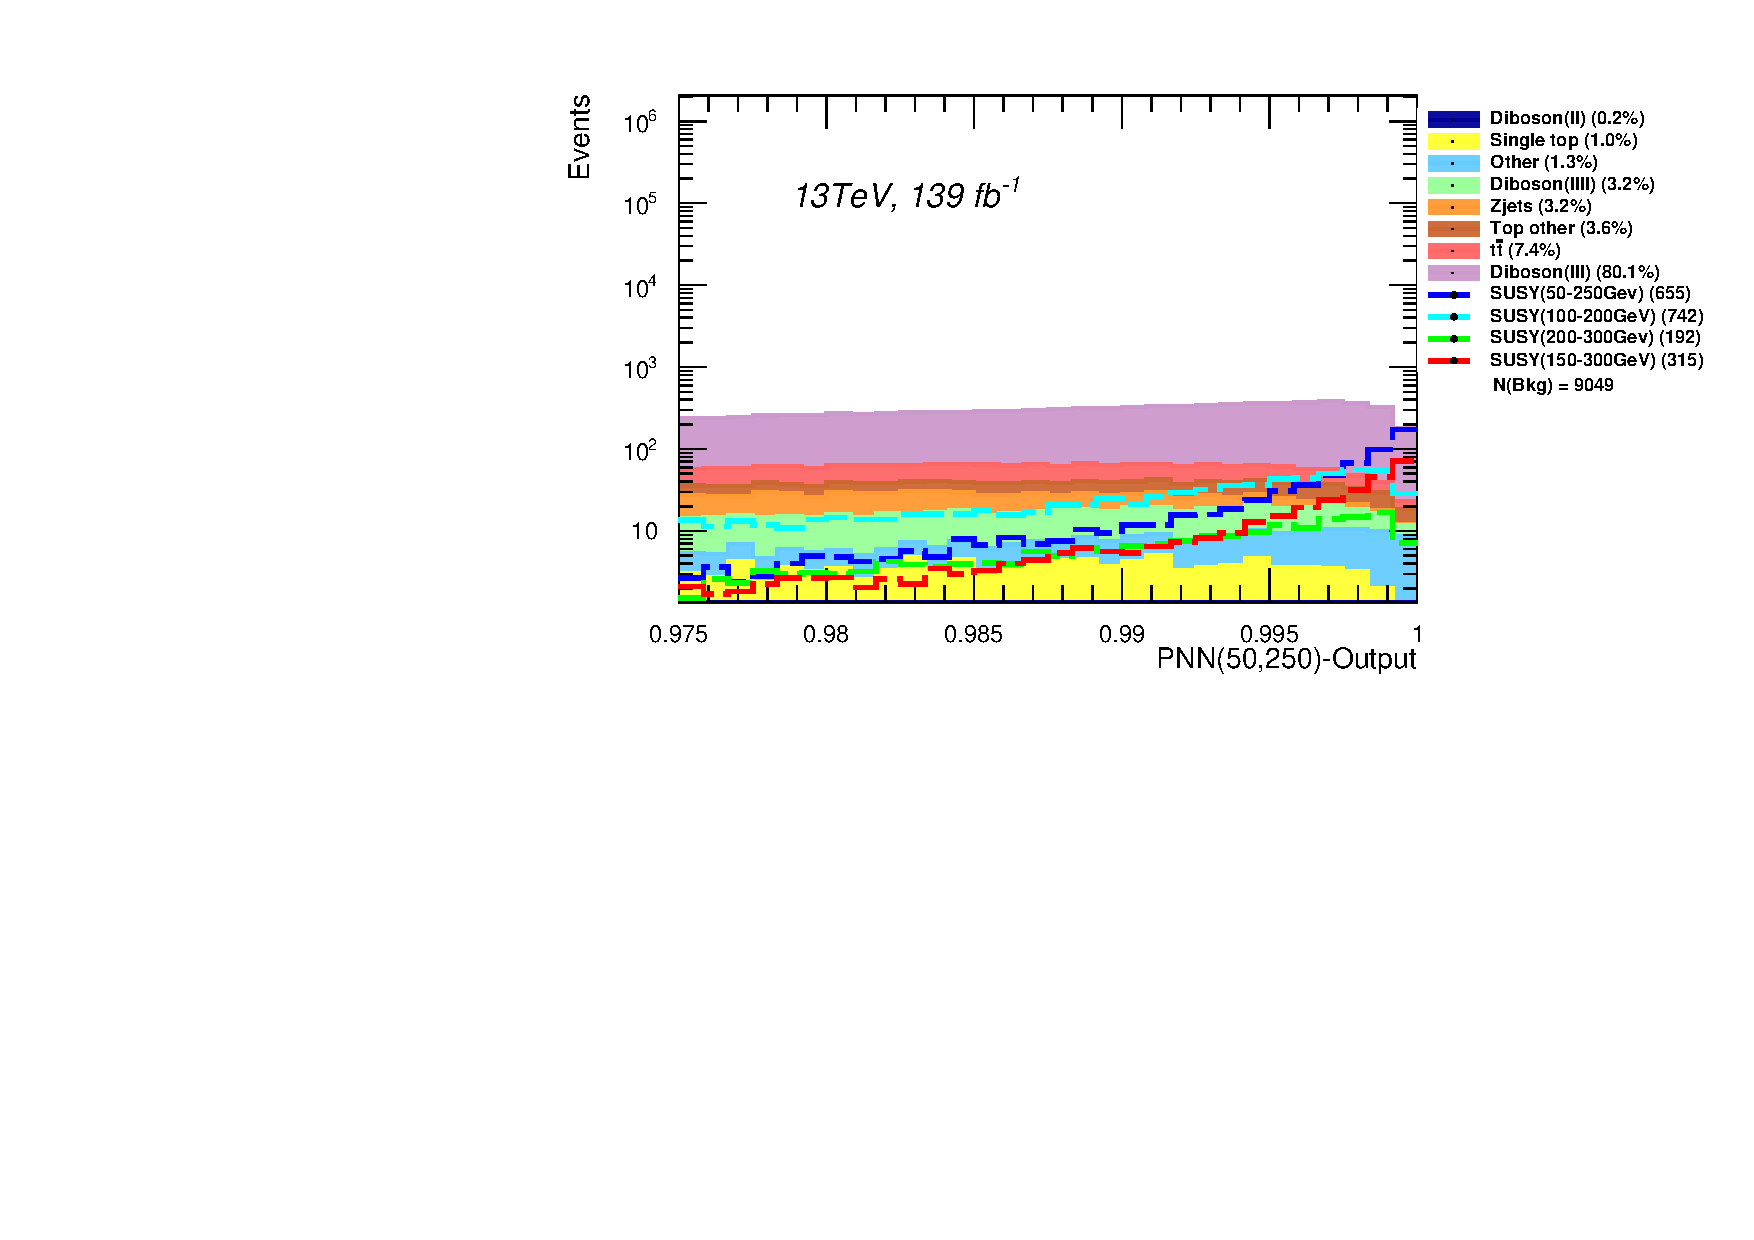
\includegraphics[width=\textwidth]{Figures/MLResults/NN/SUSY/MLDist/PNNDistTest/PNN50250Dist_C7.pdf}
        \caption{}
        \label{fig:PNN50250Dist_95}
    \end{subfigure}
    }
    \caption{}
    \label{fig:PNN50250}
\end{figure}
\begin{figure}
    \makebox[0.95\linewidth][c]{%
    \centering
    \begin{subfigure}{.45\textwidth}
        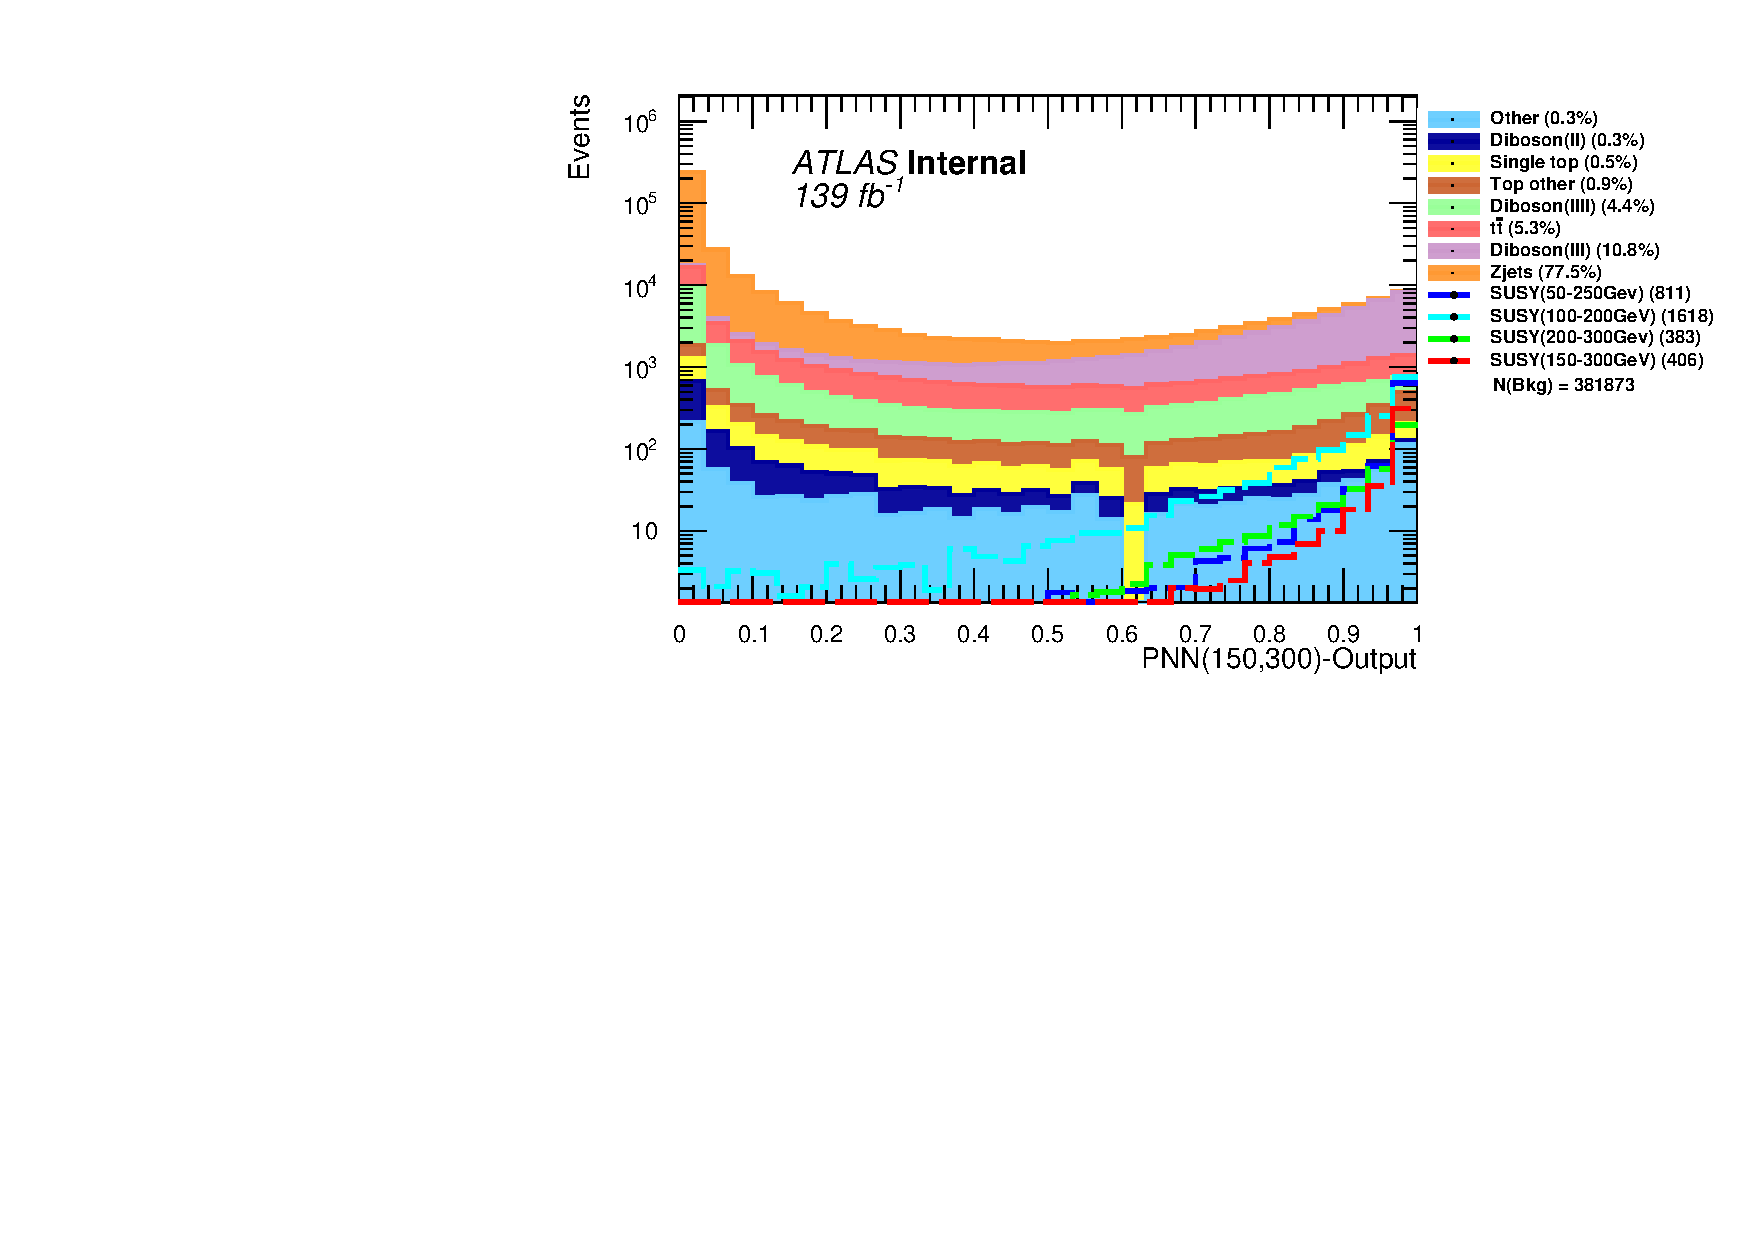
\includegraphics[width=\textwidth]{Figures/MLResults/NN/SUSY/MLDist/PNNDistTest/PNN150300Dist.pdf}
        \caption{}
        \label{fig:PNN150300Dist}
    \end{subfigure}
    \hfill
    \begin{subfigure}{.45\textwidth}
        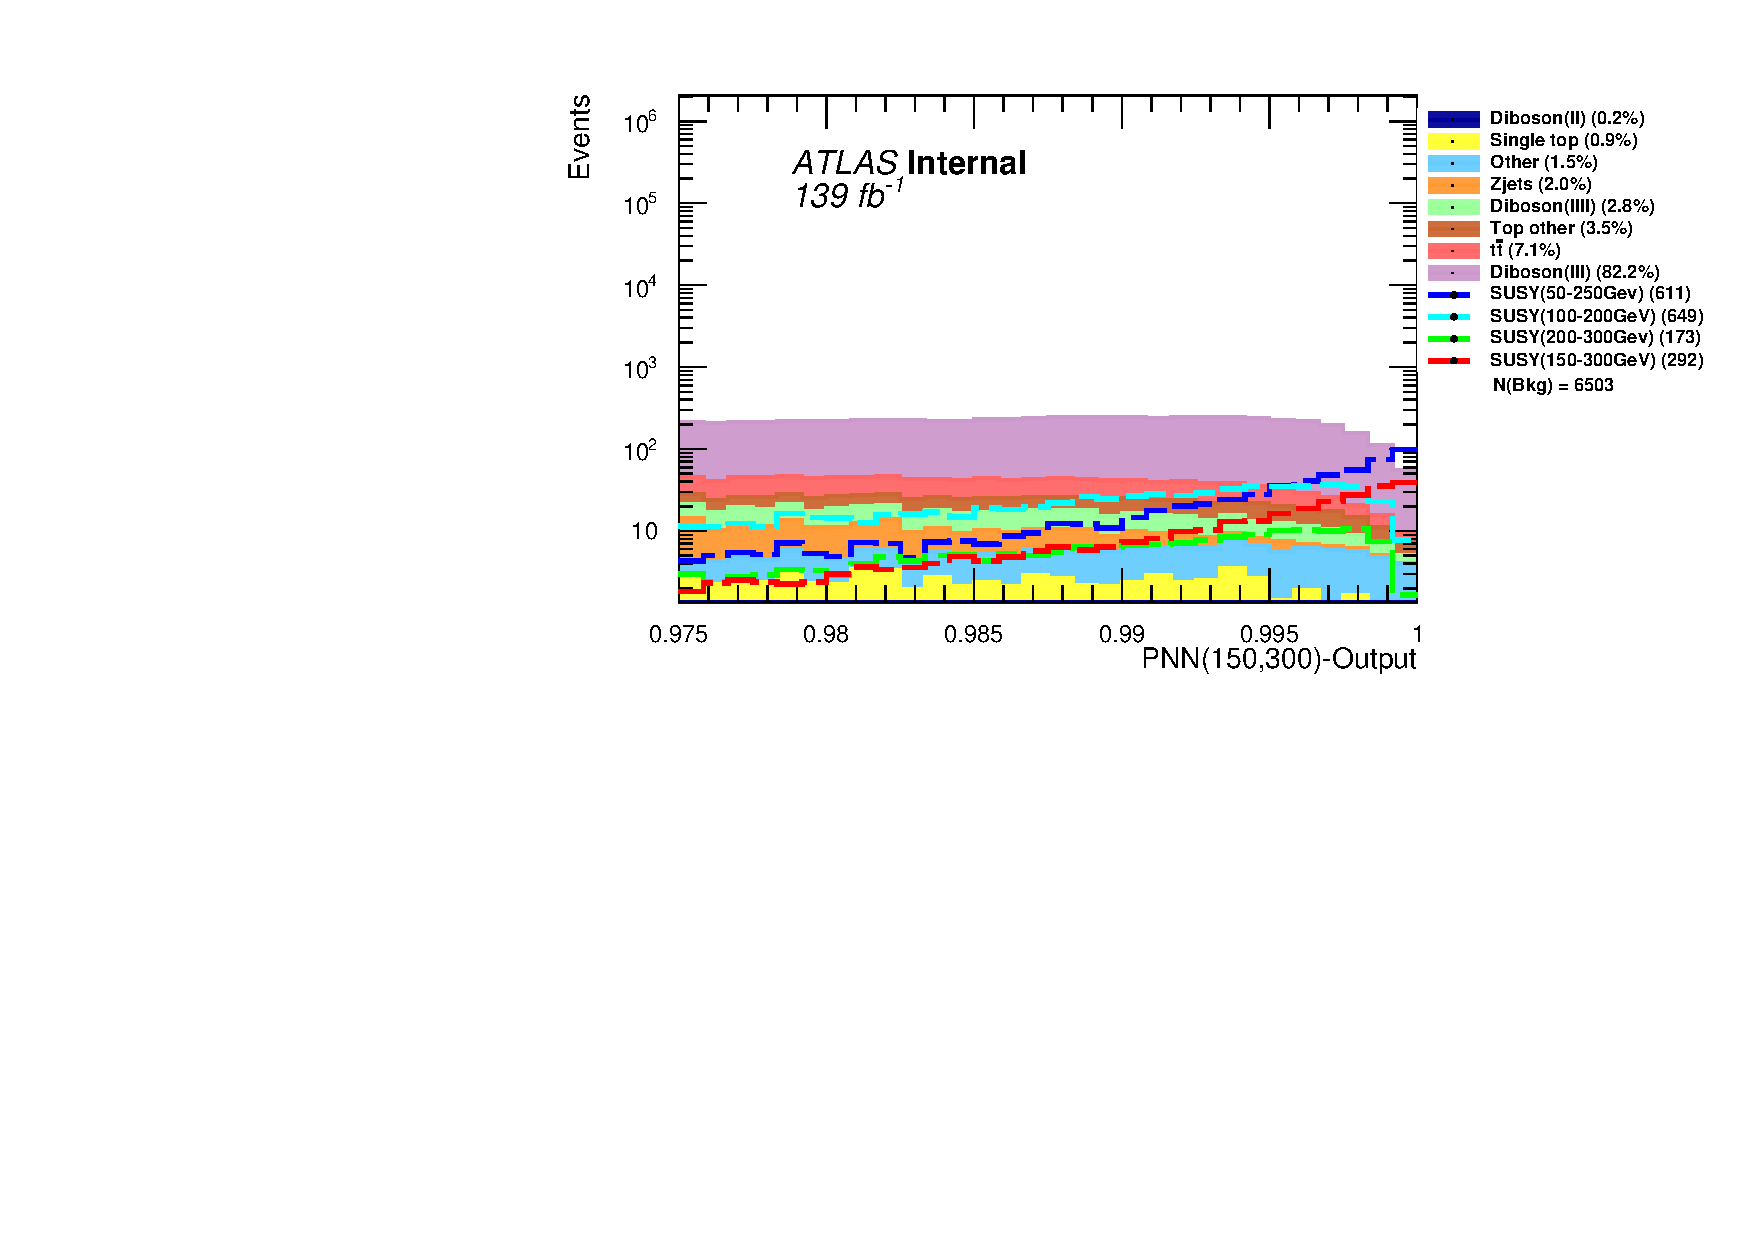
\includegraphics[width=\textwidth]{Figures/MLResults/NN/SUSY/MLDist/PNNDistTest/PNN150300Dist_C7.pdf}
        \caption{}
        \label{fig:PNN150300Dist_95}
    \end{subfigure}
    }
    \caption{}
    \label{fig:PNN150300Dist}
\end{figure}
